% CS 198 - TEMPLATE FOR EXTENDED ABSTRACT
%
\documentclass[12pt]{article}

%%% PACKAGES
\usepackage{graphicx}
\usepackage{url}
\usepackage{booktabs} % for much better looking tables
\usepackage{array} % for better arrays (eg matrices) in maths
\usepackage{paralist} % very flexible & customisable lists (eg. enumerate/itemize, etc.)
\usepackage{verbatim} % adds environment for commenting out blocks of text & for better verbatim
\usepackage{subfigure} % make it possible to include more than one captioned figure/table in a single float
\usepackage{fancyhdr} % This should be set AFTER setting up the page geometry
\pagestyle{fancy} % options: empty , plain , fancy
\renewcommand{\headrulewidth}{0pt} % customise the layout...
\lhead{}\chead{}\rhead{}
\lfoot{}\cfoot{\thepage}\rfoot{}


% Basic Variables to Set

\title{Semi-Structured Image Vectorization Through Neural Networks Based on Perception}
\author{S. F. Ballais\thanks{snballais@up.edu.ph}\\
Division of Natural Sciences and Mathematics\\
University of the Philippines Visayas \\
TACLOBAN COLLEGE}
\date{06 November 2018}

% End Variable Setting

\begin{document}
\maketitle
\tableofcontents

\pagebreak

\begin{abstract}
We describe the CSG system, a secure online portal for the Computerized Registration System of the University of the Philippines Diliman. The portal incorporates a modified one-time password scheme that allows users to utilize their university DILNET credentials to login to any of the university computing resources. We designed the system to run on top of existing authentication mechanisms and is backward-compatible. Our preliminary tests indicate that the CSG system adds a layer of security to the current authentication process without any significant computational or storage overhead.  (This paper describes a fictitious Computer Science Undergraduate Research Project at the University of the Philippines Diliman. This is only intended to show as a guide on how to write the first semester report.)
\end{abstract}


\section{Introduction}
Many images in typical use, from photographs to pixel art, are composed of pixels. Each pixel in an image contains a value that represents the colour it displays. These images are called, \textit{raster images}. This type of image are ideal when creating images that are rich and detailed. However, raster images suffer from their inability to scale well. Scaling raster images will output grainy and distorted results, sometimes even blurry ones\cite{rastervsvectorgraphics}. \textit{Vector graphics} are an alternative to raster graphics, being resolution-independent and based on objects (often called \textit{primitives}) and mathematical statements\cite{barendrecht2018locally}\cite{rastervsvector}. As a result, vector graphics generally tend to be easier to manipulate\cite{barendrecht2018locally}.

\textit{Semi-structured images} can benefit from vectorization. As defined by Hoshyari, S., et.al., these images "consists of distinctly coloured regions with piecewise continuous boundaries and visually pronounced corners". Frequently, many digital artworks, specifically computer icons, comic book imagery, and simple graphic illustrations, are considered to be semi-structured images. Many legacy semi-structured images, typically those considered to be icons and clip arts, are stored in raster formats\cite{hoshyari2018perceptiondriven}. Additionally, in manual vectorization of images, artists often have to hand-trace each stroke and region using specialized software, such as Inkscape or Adobe Illustrator, which is a labourious task\cite{matheson2018smoothing}. Automatic vectorization tools, such as Adobe Live Trace and Potrace, often demand more time rectifying the numerous tracing errors the tool produces by hand\cite{matheson2018smoothing}, and does not always produce results aligned with human perception\cite{hoshyari2018perceptiondriven}. Most vectorization algorithms are geared towards natural images (i.e. photographs) which frequently produce results not aligned with human expectations on artist-drawn imagery\cite{hoshyari2018perceptiondriven}. These cases call for a robust vectorization algorithm for semi-structured images that produces outputs that primarily align well with human-perceived results  As noted by Hoshyari, S., et. al., human observers have a clearer mental image of the expected vector result from a raster semi-structured data. As such, vectorization results of semi-structured images require to be as close as possible to the mental image produced by humans\cite{hoshyari2018perceptiondriven}.

Due to the fact that semi-structured images consists of distinct regions based on colour, the general flow of vectorizing semi-structured images can simply be boiled down into extracting those distinct regions and their boundaries, performing vectorization on those boundaries and appropriately colouring them, and combining the resulting vectors into a single vector object. The major technical challenge for this is vectorizing the region boundaries via piecewise free-form vector curves\cite{hoshyari2018perceptiondriven}. The most recent work on this topic is that of Hoshyari, S., et. al. Their work revolves primarily on accuracy and two key principles of Gestalt psychology: \textit{simplicity}, and \textit{continuity}. Simplicity simply states that human observers prefer simpler interpretations of geometric interpretations of raster images. Continuity states that human observers have a tendency to group stimuli into one continuous curves and patterns. Jagged raster boundaries are perceived to be piecewise smooth curves in their vector forms. In addition, observers would only mentally segment boundaries at a small set of discontinuous corners. Their work, however, becomes computationally expensive on larger inputs. Despite utilizing a corner classifier developed via machine learning as part of their vectorization, their classifier still produces results that require them to have an additional processing step, called \textit{corner removal}, to produce better results.

I propose a method that is an improvement of the work done by Hoshyari, S. et. al. by improving the corner classifier in an attempt to render the corner removal step unnecessary, and utilizing machine learning to automatically draw the appropriate vector curves and lines, without relying on greedily computing and fitting the appropriate curves on the region boundaries. The latter, of which, is the method utilized in the framework devised by Hoshyari, S., et. al., which, as stated earlier, is computationally expensive at higher image resolutions.

\section{Image Vectorization}
The ability to provide high quality and clear resolution-independent images is the strong point of vector graphics. From any display, and any resolution, vector images still look crisp and no loss of details. Vectorization consists of various algorithms, heuristics, data structures, and geometric primitives that work together to generate a vector output from a raster input. Previous works on image vectorizations deal with various input images from pixel art to natural images. All of which have varying degrees of success in vectorization depending on the input. In the pursuit of supporting higher resolutions, previous works have also delved with upscaling raster images rather than converting to their vector versions.

\subsection{Previous Works}
\subsubsection{Image Upscaling}
Image upscaling is the process of increasing the resolution of low-resolution raster images. The process utilizes single-image super resolution (SISR) algorithms to perform the transformation. There are many SISR algorithms that have been developed that focus on specific image classes such as faces, and graphics artwork. However, generic SISR algorithms exist as well to work for all kinds of images \cite{SISRBenchmark}. Examples of these generic SISR algorithms include Nearest-Neihbour, Lancosz, and Bicubic Interpolation \cite{DepixelizingPixelArt}. As a side note, many raster editing software such as Adobe Photoshop and GIMP use bicubic interpolation or provided as an option (default in the aforementioned software packages) when transforming, i.e. resizing (in common terms), images. These generic SISR algorithms, being generic, assume nothing about the underlying data (aside from being band-limited), which results in blurring of edges and ring artifacts \cite{DepixelizingPixelArt}.

\subsubsection{Natural Image Vectorization}
One of the most common applications of vectorization is the vectorization of \textit{natural images}. Natural images are essentially photographs. They contain continuous colour tones and fine details at the pixel level. Commercial packages employ natural image vectorization methods. Hoshyari, S. \cite{hoshyari2018perceptiondriven} notes that natural image vectorization methods addresses two separate challenging problems: image segmentation and segment boundary fitting. Most methods focus on the former and perform operations such as lossy moothing that is undesirable for inputs with perceptually well-defined boundaries designed by artists such as those in semi-structured images. Depending on the algorithm used, the vectorization results of natural images may or may not be satisfactory, as shown in Figure 1. Basing from the figure, the resulting outputs either may lose quality or details, or result in a larger file size.

\begin{figure}[h]
\centering
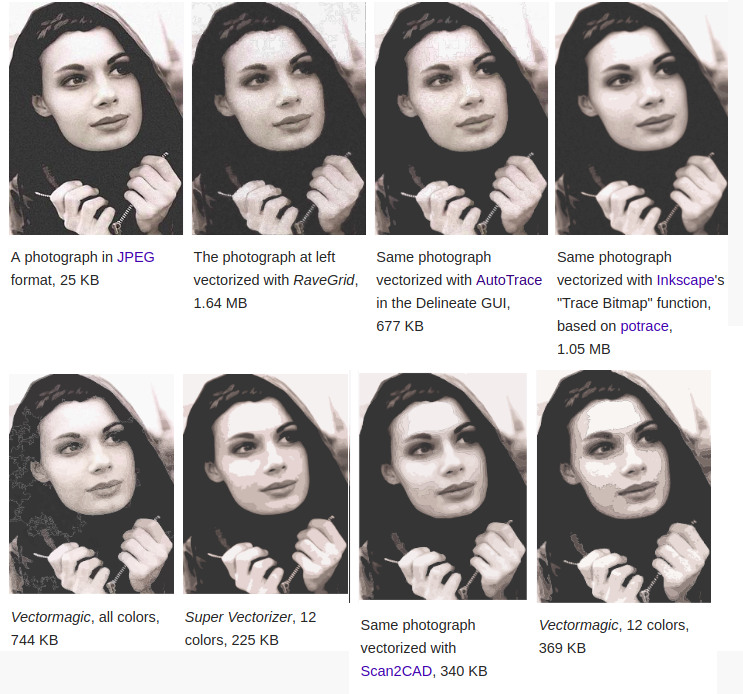
\includegraphics[scale=2.0]{images/natural-vectorization.png}
\caption{Outputs of various vectorization algorithms in vectorizing a natural image. Acquired from Wikipedia \(https\://en.wikipedia.org/wiki/Image\_tracing\).}
\label{fig:natural-vectorization}
\end{figure}

Other image vectorization techniques that can handle natural images uses a geometric primitive called a \textit{gradient mesh}. As defined by Sun, J., et. al. \cite{ImageVectorizationOptimizedGradientMeshes}, Gradient meshes are geometric primitives that consist of topologically planar Ferguson patches with mesh-lines and has four boundaries, each of which consists of one or more cubic Bezier splines. Gradient meshes allow for multiple colours to be rendered with smooth transitions in a single primitive. This leads to image vectorizations that capture details and are close to their raster counterparts. Some image information such as fine details and highly textured regions may fail to be captured by gradient meshes \cite{ImageVectorizationOptimizedGradientMeshes}. Recent researches have improved gradient meshes, such as extending them with mathematically exact local refinement, branching capabilities, and sharp colour transitions, as was done in the work of Barendrecht, P., et. al. \cite{barendrecht2018locally}. However, since we are dealing with vectorizing semi-structured images, which do not contain gradients, we will not be utilizing gradient meshes in this paper.

\subsubsection{Vectorization of Artist-Generated Images}
% Discuss vectorization of semi-structured images.
% Discuss how we can categorize/define artist-generated images to involve pixel art and semi-structured images.

\subsection{Accompanying Technologies}


\section{Problem Statement}

State here, in detail what you will be working on.

You can follow the format below:

We are developing a {\it describe your project here}\\
in order to {\it describe the problem you are addressing}\\
because {\it describe the gap(s) that you have identified}.

You can revise the wording, you do not need to use the wording I have given. It is just a suggestion on the structure.

Here is a concrete example.

We are designing a disaster management system for flooding that allows for clustering, aggregation and filtering of data entries in order to improve the visualization and report generation of current flood hazard mapping systems. Some current solutions employ proprietary algorithms resulting in exorbitant system costs. Some of the more inexpensive options do not provide data checking and filtering, requiring manual intervention to check each and every data entry. Our solution provides for an accessible system that automatically checks each data entry and flags those that are possibly erroneous for manual verification. 

You can also discuss here your constraints, i.e., what your thesis will not tackle.

This is how you should cite a work ~\cite{Nobody06}. The entries will be in a separate file (we have named it mybib.tex in this example). 

Here is another citation ~\cite{Reyes2010}. 


\section{Proposed Methodology}

Discuss here how you plan to develop the system. Discuss your design here.

What components are you using.
What algorithms.
What API libraries.

This is your WHOLE PLAN - not just what you have finished so far.

This is how you include a graphics file 

This is how to reference the figure. See Figure ~\ref{fig:xenlogo} for the Xen logo image. 

\section{Preliminary Results}
Discuss what you have done so far. This should be a subset of your Proposed Methodology.

\bibliography{mybib}{}
\bibliographystyle{plain}


\end{document}